\begin{figure}[ht!]
\centering
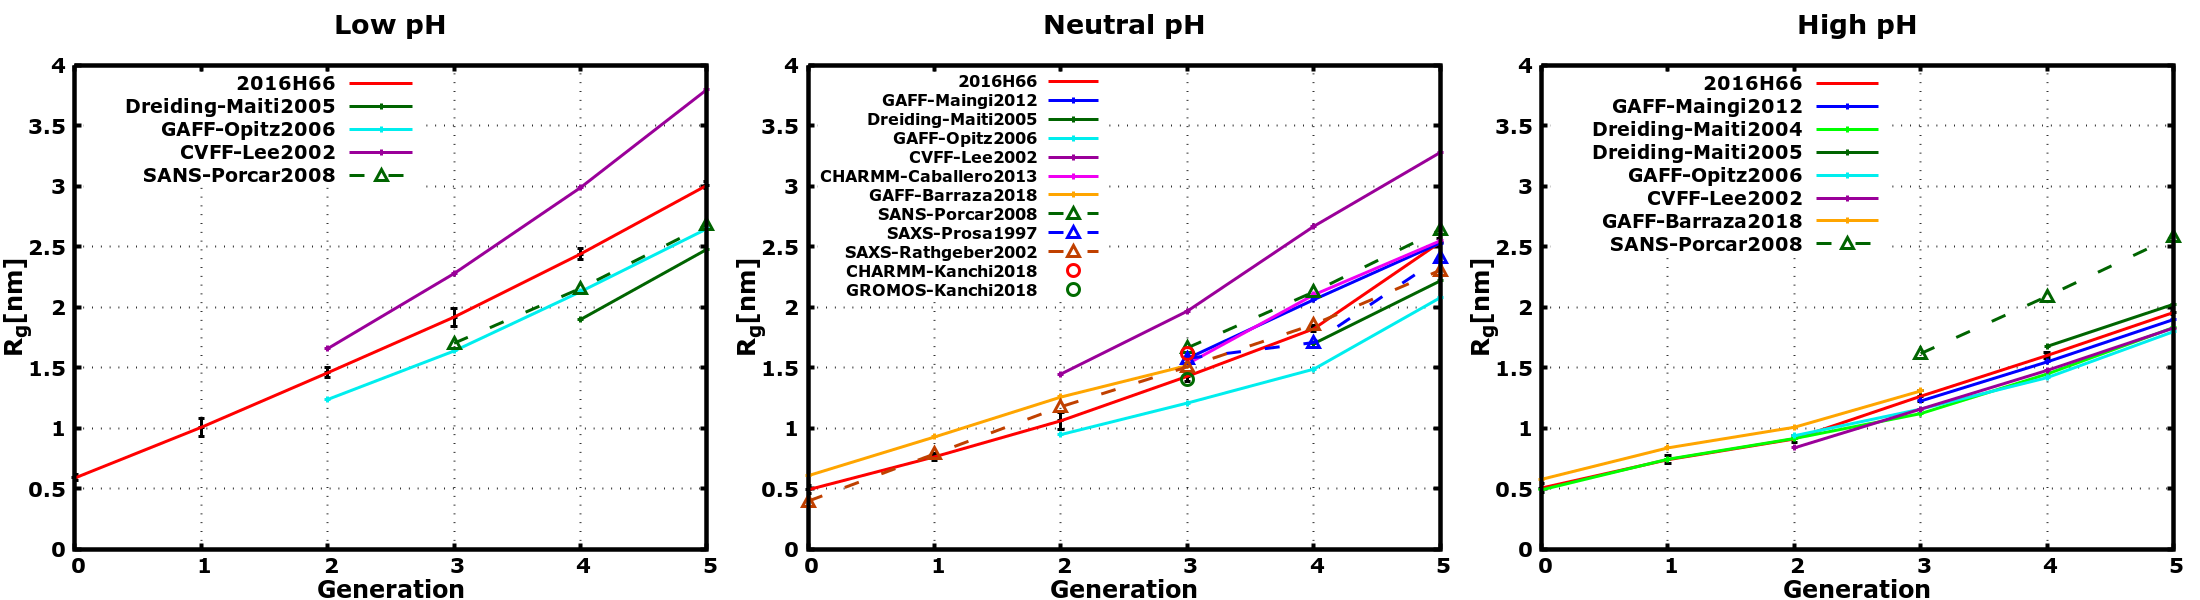
\includegraphics[width=\textwidth]{images/PME/PAMAMRg.png}
\caption{Raio de giro ($R_g$) em função da geração em meios de pH baixo (imagem da esquerda), neutro (imagem do meio) e alto (imagem da direita).
Os resultados obtidos com o campo de força 2016H66\cite{Horta2016} são comparados com resultados de estudos experimentais e de simulações prévios:
Prosa1997\cite{Prosa1997}, %\cite{PR97.2},
Lee2002\cite{Lee2002}, %\cite{LE02.8},
Caballero2013\cite{Caballero2013}, %\cite{CA13.4},
Rathgeber2002\cite{Rathgeber2002}, %\cite{RA02.6},
Maiti2005\cite{Maiti2005}, %\cite{MA05.26},
Opitz2006\cite{Opitz2006}, %\cite{OP06.1},
Porcar2008\cite{Porcar2008}, %\cite{PO08.3},
Maiti2009\cite{Maiti2009}, %\cite{MA09.18},
Maingi2012\cite{Maingi2012}, %\cite{MA12.23},
Barraza2018\cite{Barraza2018}, %\cite{BA18.Y},
Kanchi2018\cite{Kanchi2018}.} %\cite{KA18.Y}.}
\label{supfig:PAMAMRg}
\end{figure}

\begin{figure}[ht!]
\centering
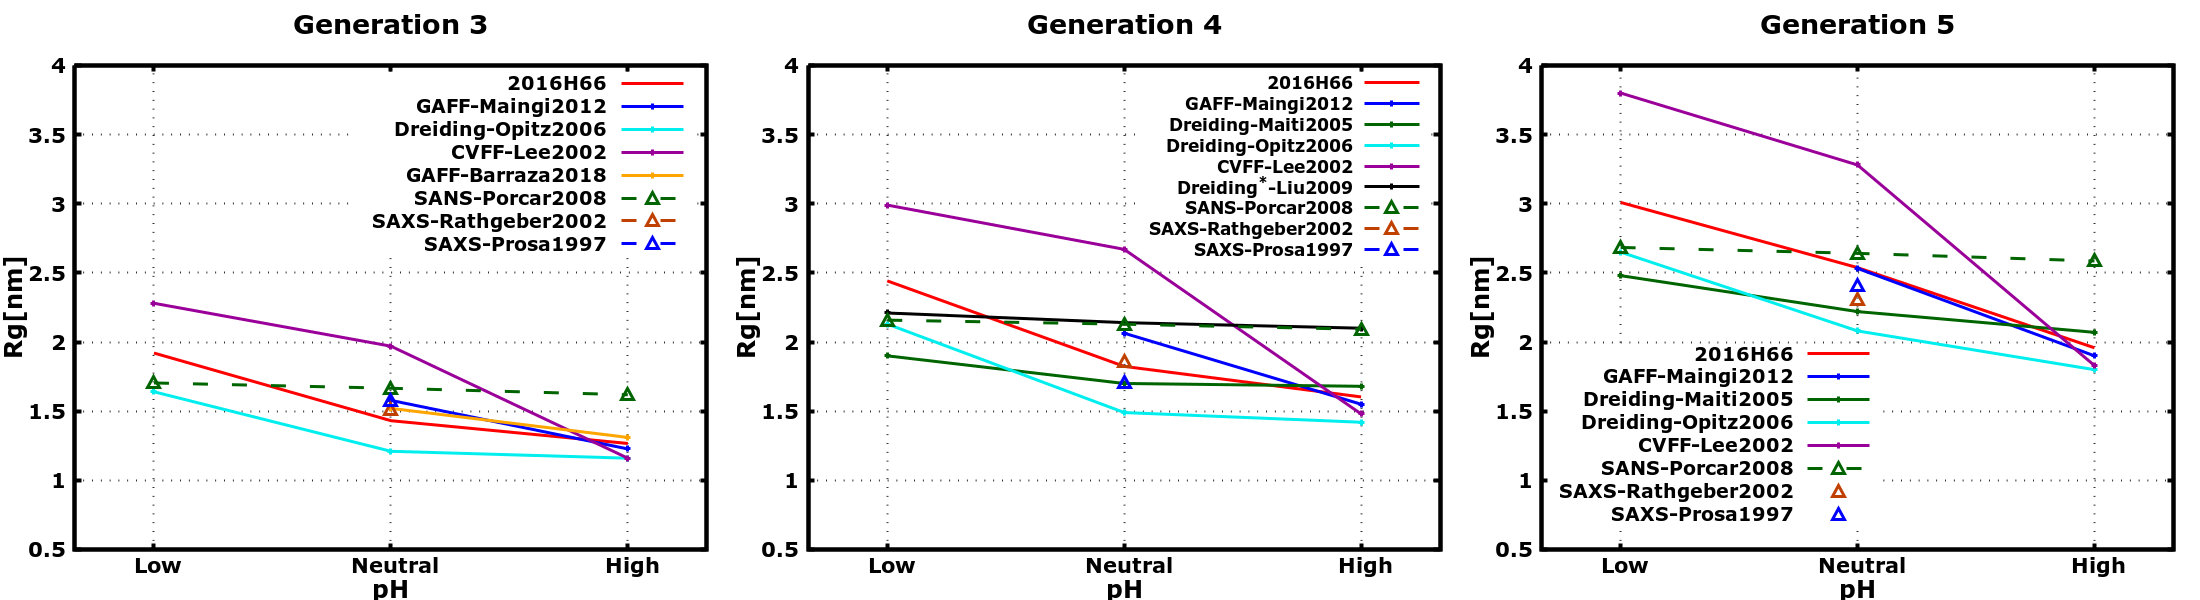
\includegraphics[width=\textwidth]{images/PME/PAMAMgyrateGpH.png}
\caption{Raio de giro ($R_g$) em função do pH para o PAMAM de geração 3 (imagem da esquerda), 4 (imagem do meio) e 5 (imagem da direita).
Os resultados obtidos com o campo de força 2016H66\cite{Horta2016} são comparados com resultados de estudos experimentais e de simulações prévios:
Prosa1997\cite{Prosa1997}, %\cite{PR97.2},
Lee2002\cite{Lee2002}, %\cite{LE02.8},
Rathgeber2002\cite{Rathgeber2002}, %\cite{RA02.6},
Maiti2005\cite{Maiti2005}, %\cite{MA05.26},
Opitz2006\cite{Opitz2006}, %\cite{OP06.1},
Porcar2008\cite{Porcar2008}, %\cite{PO08.3},
Liu2009\cite{Liu2009}, %\cite{LI09.Y},
Maingi2012\cite{Maingi2012}, %\cite{MA12.23}.  }
Barraza2018\cite{Barraza2018}.} %\cite{BA18.Y},
\label{supfig:PAMAMRgpH}   
\end{figure}

\begin{figure*}[ht!]
\centering
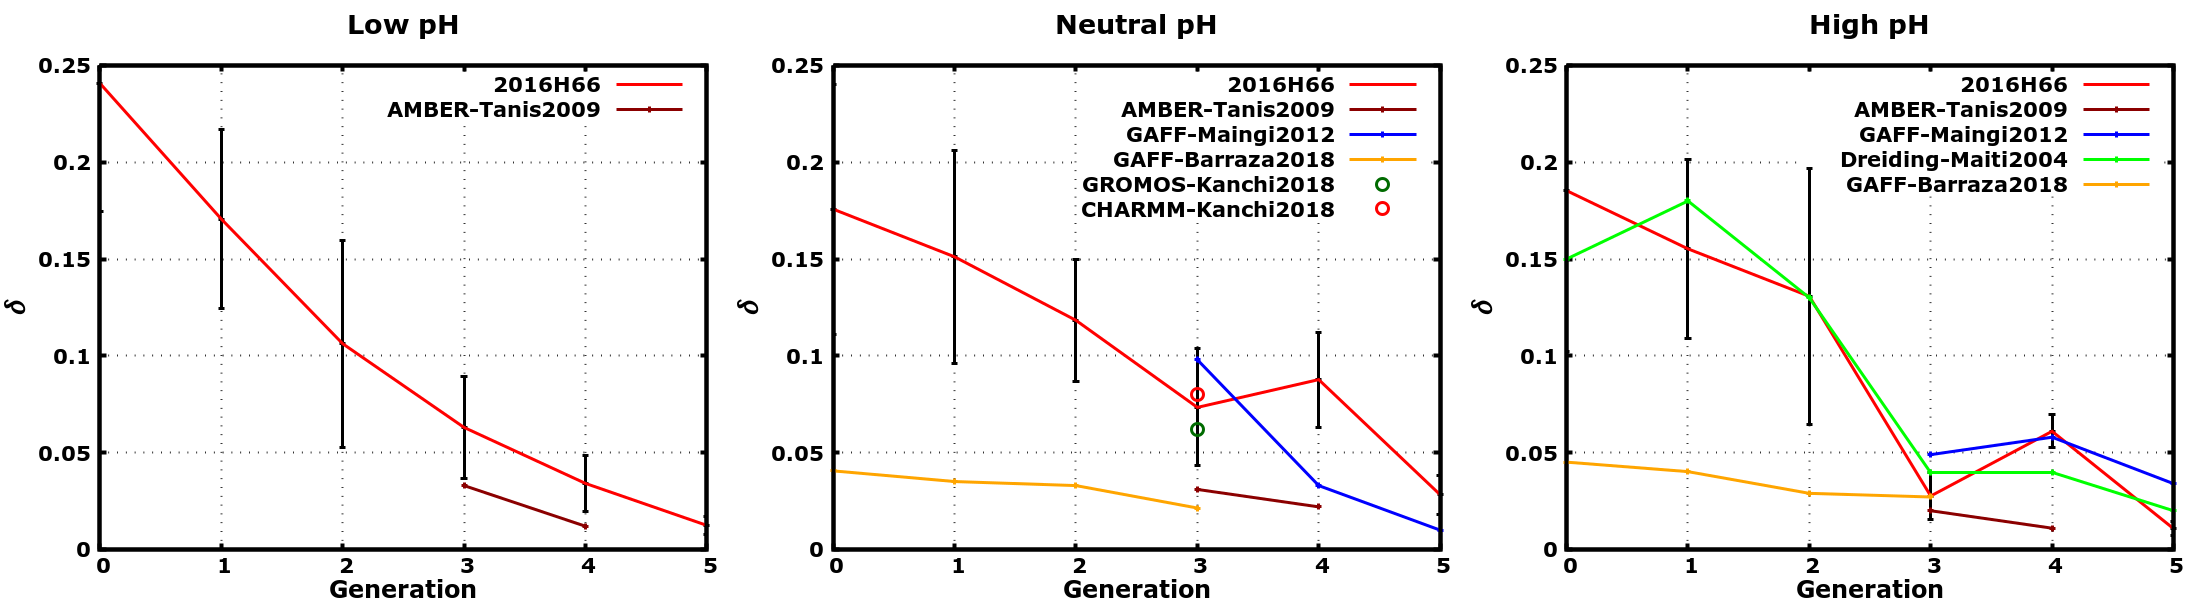
\includegraphics[width=\textwidth]{images/PME/PAMAMAsphericity.png}
\caption{Asfericidade $\delta$ do PAMAM em função da geração. As curvas da esquerda para a direita mostram, respectivamente, os sistemas em baixo, neutro e alto pH.
Os resultados obtidos com o campo de força 2016H66\cite{Horta2016} são comparados com resultados de estudos experimentais e de simulações prévios:
Maiti2004\cite{Maiti2004}, %\cite{MA04.18},
Tanis2009\cite{Tanis2009}, %\cite{TA09.6},
Maingi2012\cite{Maingi2012}, %\cite{MA12.23},
Freire2016\cite{Freire2016}, %\cite{FR16.Y}.}
Barraza2018\cite{Barraza2018}.} %\cite{BA18.Y} and
\label{supfig:PAMAMAsphericity}
\end{figure*}

\begin{figure*}[ht!]
\centering
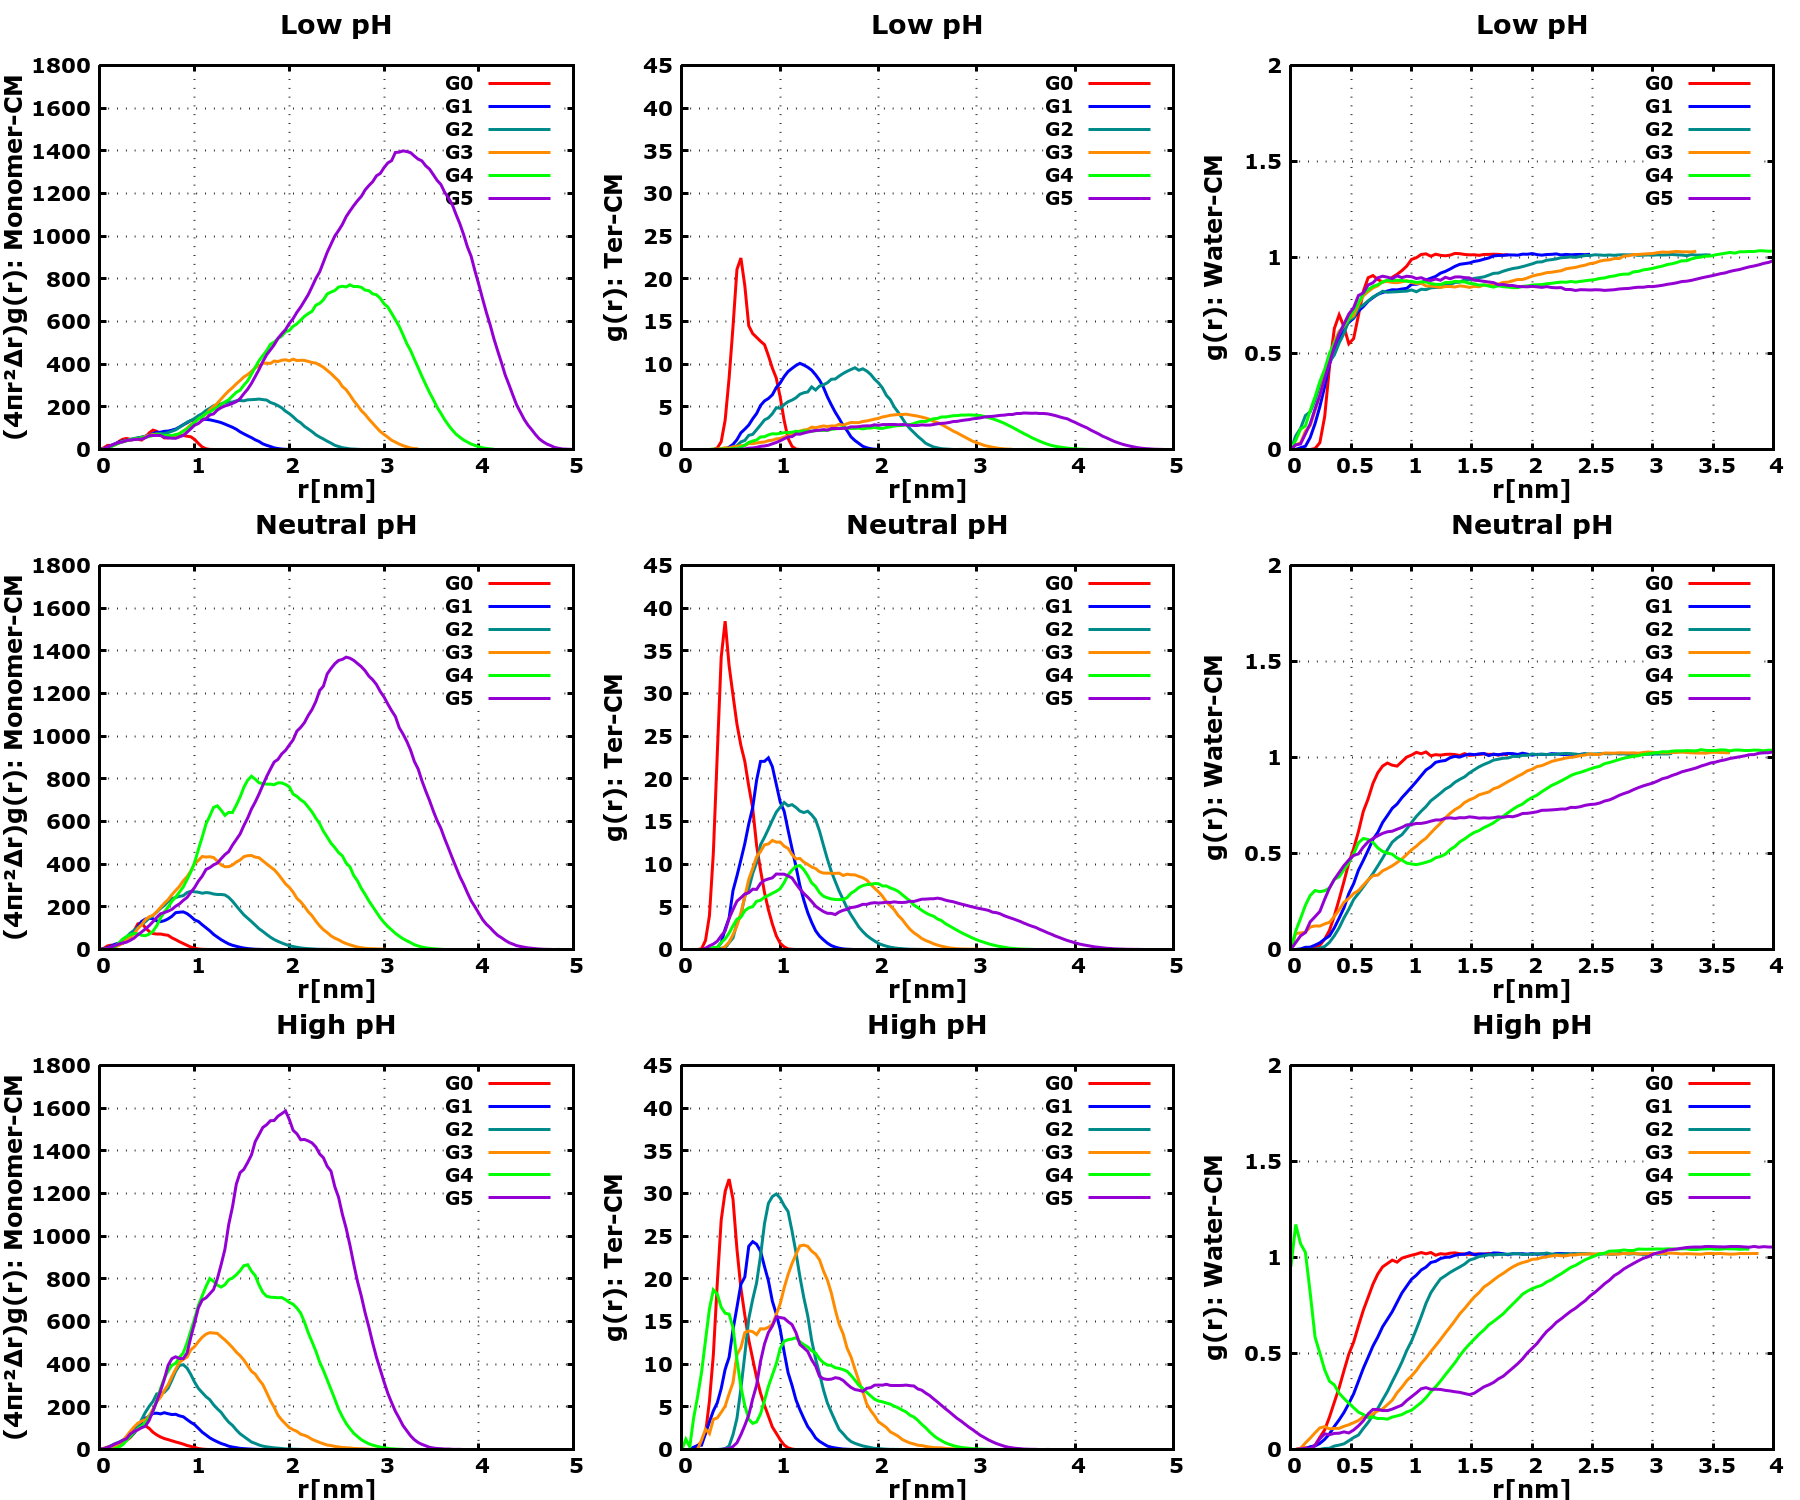
\includegraphics[width=\textwidth]{images/PME/PAMAMRDF.png}
\caption{Função de distribuição radial (RDF) $g(r)$ para o PAMAM. As curvas da esquerda, do meio e da direita mostram, respectivamente, as RDFs do centro de massa do dendrímero em relação à todos os átomos do dendrímero, às aminas primárias terminais e às moléculas de água. E as linhas superiores, intermediárias e inferiores mostram os RDFs descritos anteriormente em condições de pH baixo, neutro e alto, respectivamente. A coluna da esquerda não foi normalizada pelo volume da camada esférica utilizada.}
\label{supfig:PAMAMRDF}
\end{figure*}

\begin{figure*}[ht!]
\centering
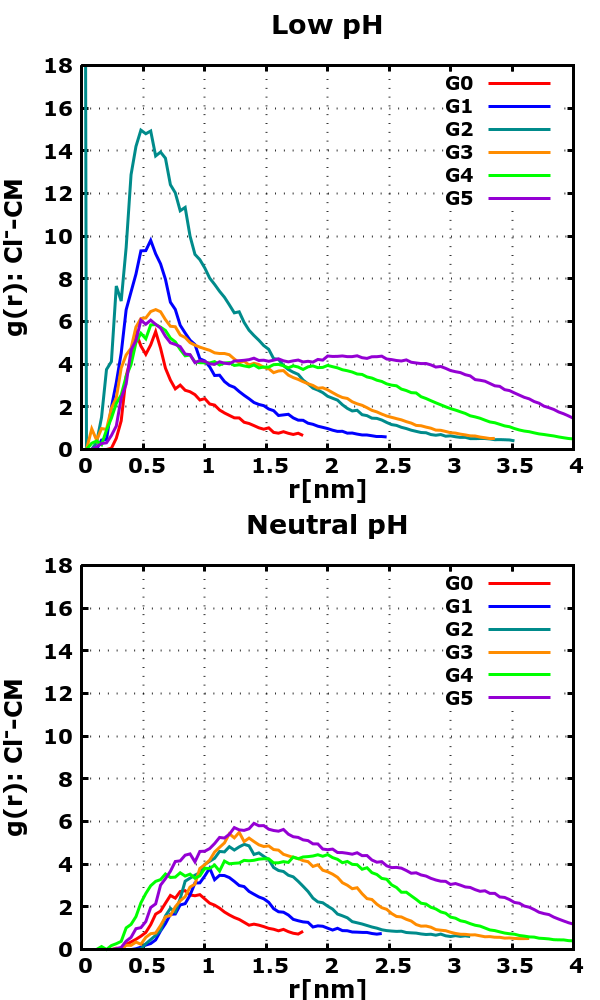
\includegraphics[scale=0.3]{images/PME/PAMAMClRDF.png}
\caption{Função de densidade radial $g(r)$ para o PAMAM. As curvas mostram o RDF de contra-íons Cloreto em relação ao centro de massa do dendrímero para os casos onde o contra-íon está presente(pHs alto e neutro).}
\label{supfig:PAMAMClRDF}
\end{figure*}